\chapter[Processo]{Processo}

Foi adotado um processo de engenharia de requisitos hibrido, utilizando aspectos do SAFe e do RUP .

O SAFe é um processo baseado nos princípios do desenvolvimento ágil, no pensamento Lean e no fluxo de desenvolvimento de produtos, tendo como foco principal as pessoas envolvidas durante o processo e o produto a ser entregue.

Três níveis organizacionais compõem o SAFe, o nível de Portfólio ou estratégico, o nível de programa também referido como tático e por fim o nível de time ou operacional, baseando-se nos seguintes princípios:

\begin{itemize}
	\item Visão Sistêmica;
	\item Economia da Cadeia de Valor;
	\item Desenvolver Iterativamente e Incrementalmente;
	\item Rápida adaptação;
	\item Testes e Integrações frequentes;
	\item Gerencia de Riscos através de ciclos de aprendizado;
	\item Sincronia entre os domínios, o planejamento e a colaboração;
	\item Marcos são baseados na avaliação objetiva dos sistemas de trabalho;
	\item Tomada de decisão descentralizada.
\end{itemize}


O RUP ou processo unificado é um processo proprietário de engenharia de software que fornece técnicas a serem seguidas pela equipe de desenvolvimento de software, a fim de aumentar sua produtividade.

O RUP eh um processo orientado a objetos e eh projetado e documentado utilizando notação UML para ilustrar seus processos.

Cinco componentes principais compõem o RUP:

\begin{itemize}
	\item \textbf{Fluxos de Trabalho:} É o passo a passo do que o envolvido deve seguir para desenvolver uma atividade.
	\item \textbf{Atividades:} Apresenta o trabalho que deve ser exercido por um membro da equipe apos está consciente do seu papel no decorrer do projeto. 
	\item \textbf{Artefatos:} É o produto de trabalho de uma atividade, também pode servir de insumo para mesma.
	\item \textbf{Disciplinas:} É um conjunto de atividades que fazem parte de um mesmo grupo.
	\item \textbf{Papéis:} Apresenta a responsabilidade do envolvido em certa atividade.
\end{itemize}

A figura \ref{fig:processo} seguinte mostra a visão geral do processo formado durante a execução do trabalho, e as figuras 2 e 3 ilustram o subprocesso de desenvolvimento e a gerencia de mudança respectivamente.


\begin{figure}[H]
    \centering
	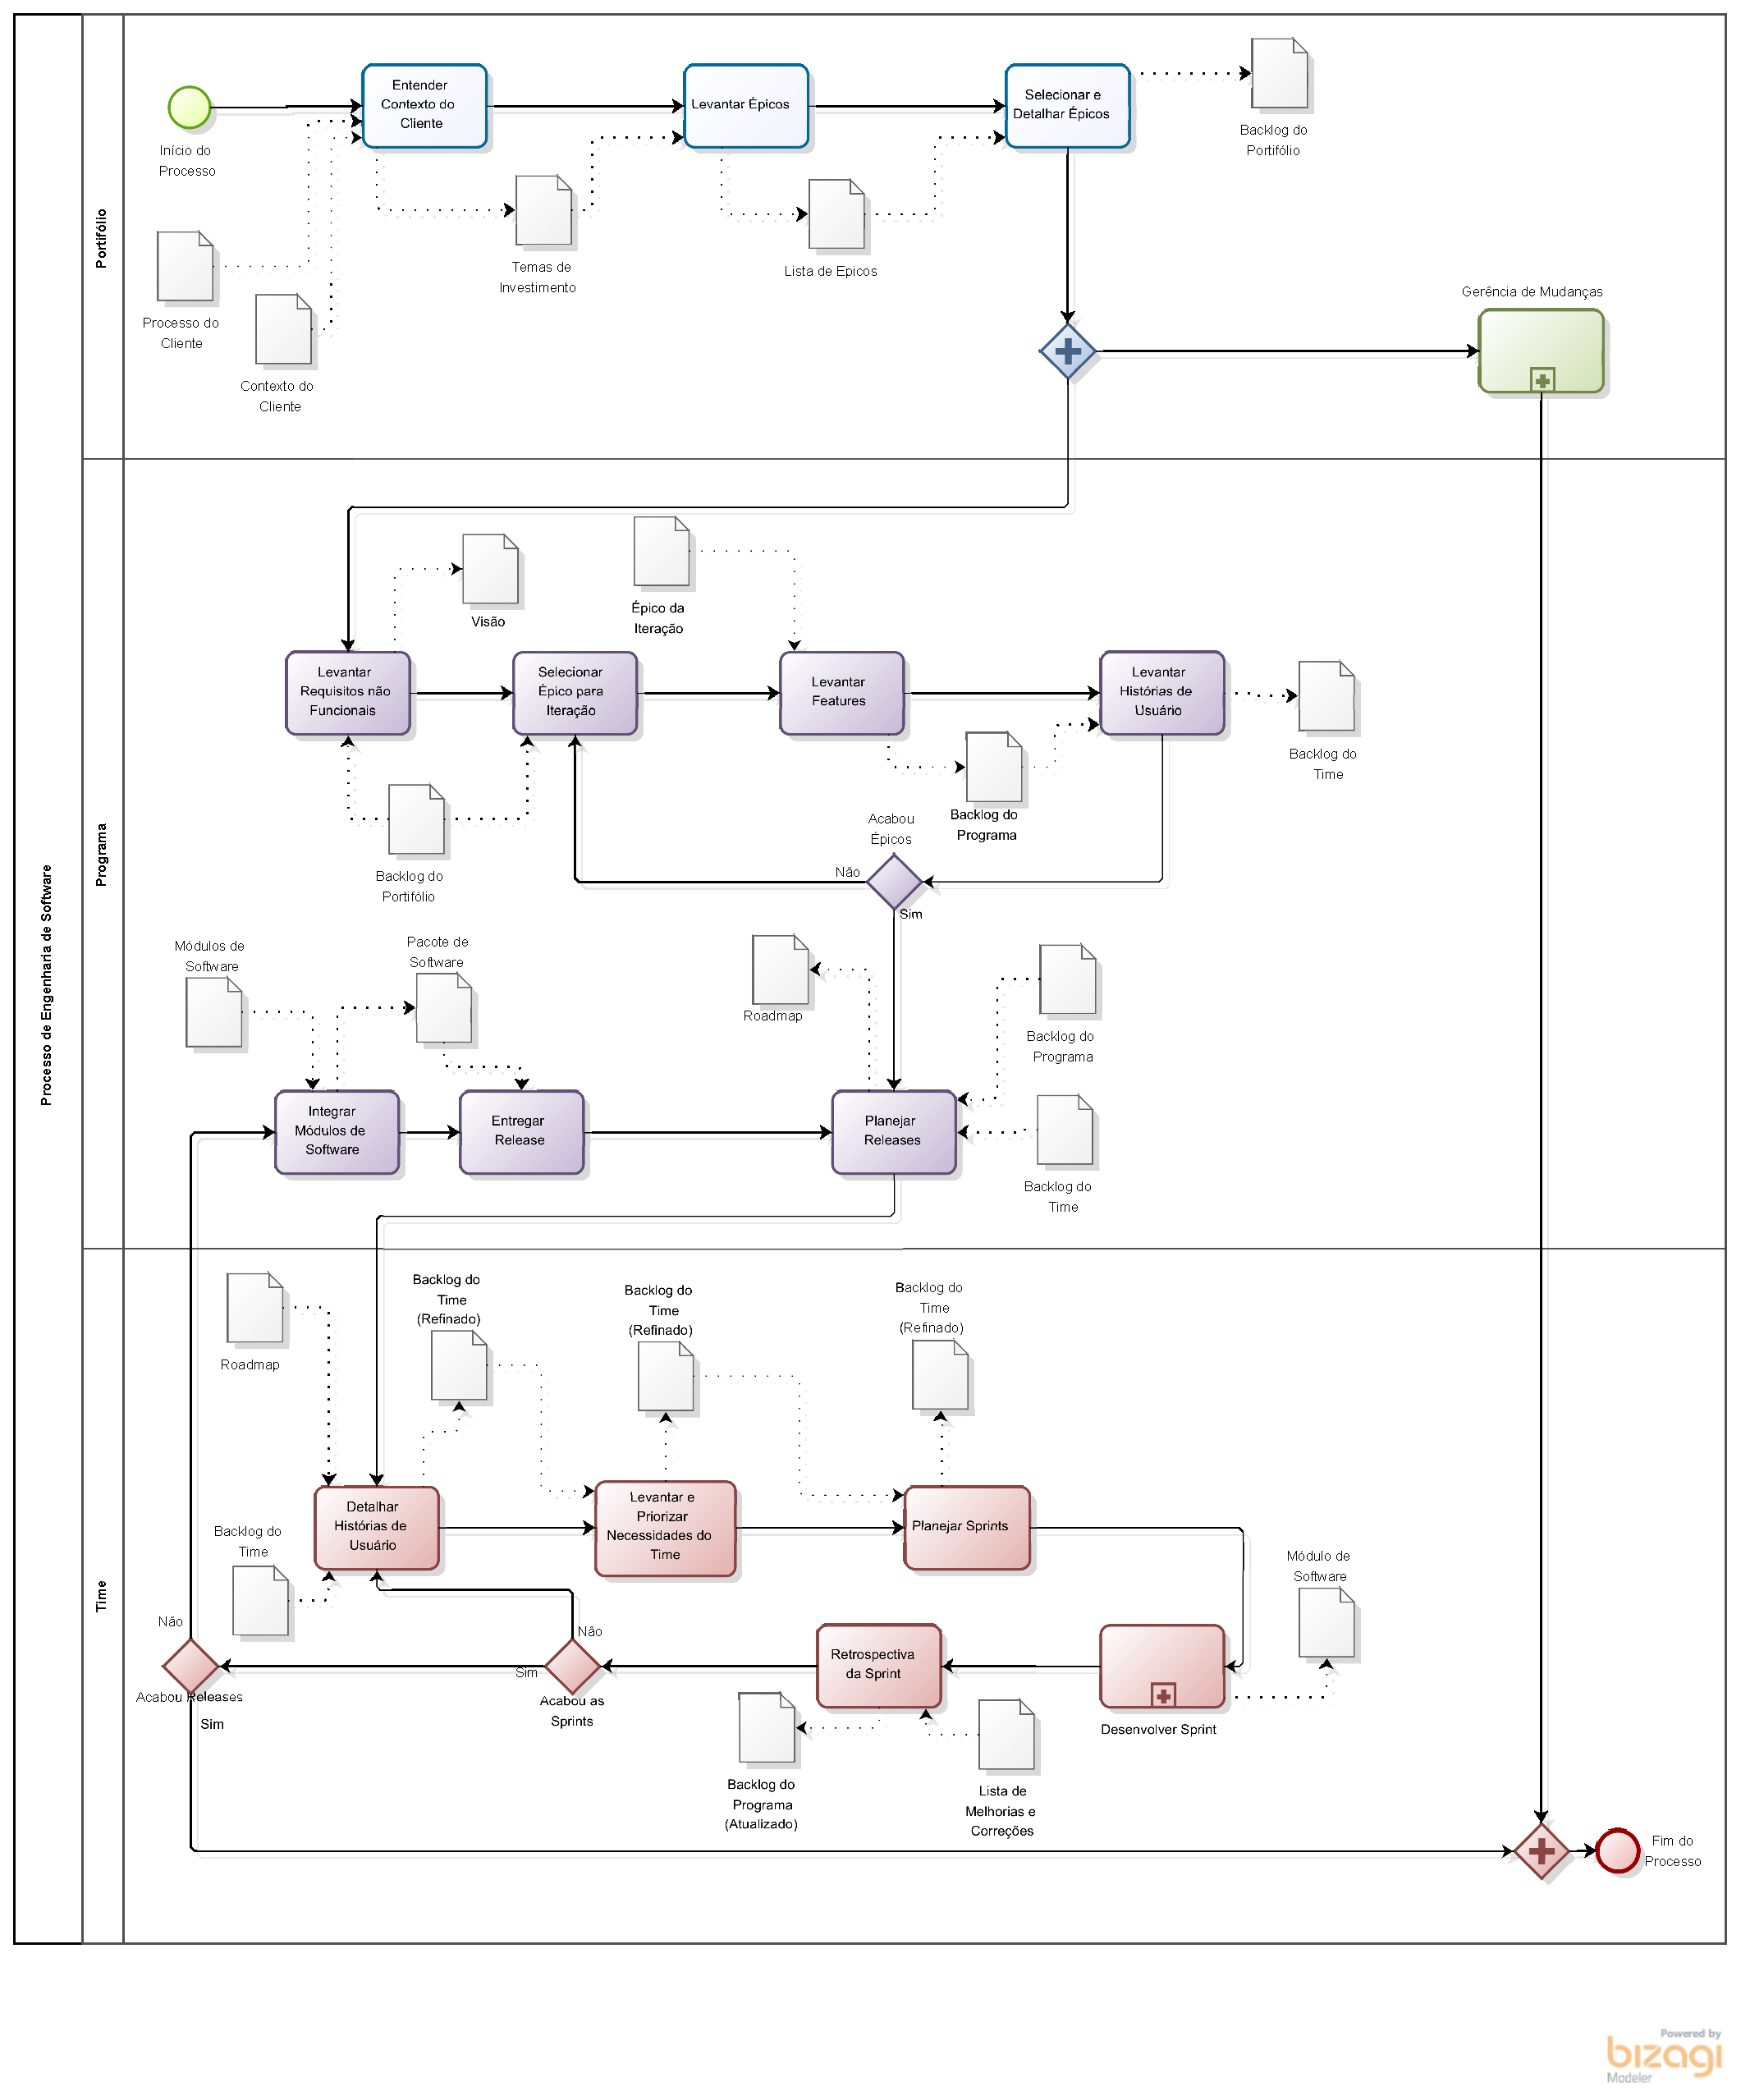
\includegraphics[trim = 0mm 25mm 0mm 0mm,clip,keepaspectratio=true,scale=0.5]{figuras/processo_req.eps}
    \caption{Processo de Engenharia de Requisitos}
    \label{fig:processo}
\end{figure}

\begin{figure}[H]
    \centering
	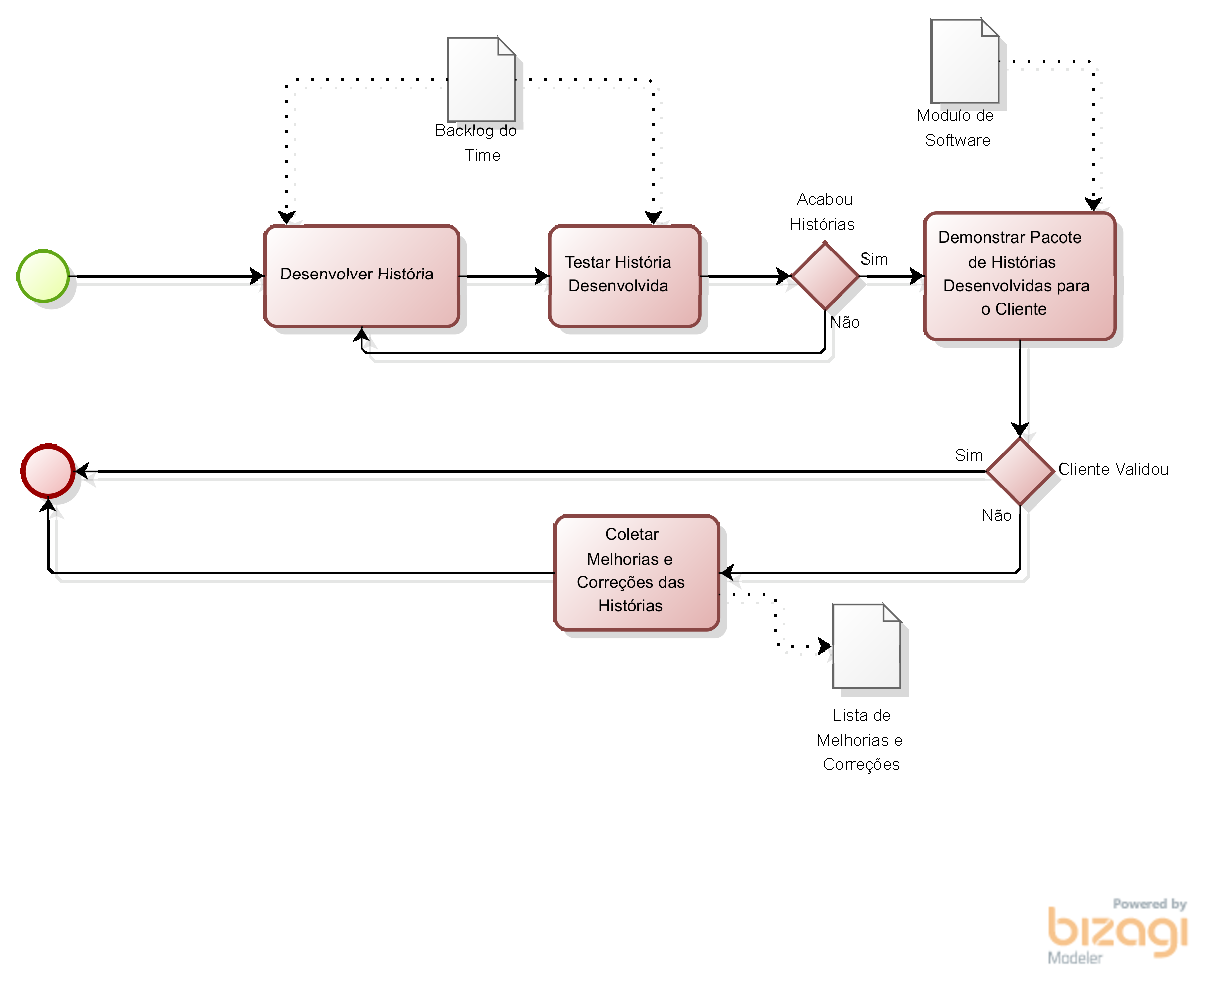
\includegraphics[keepaspectratio=true,scale=0.5]{figuras/desenvolves.eps}
    \caption{Subprocesso de Desenvolvimento}
    \label{fig:processo}
\end{figure}

\begin{figure}[H]
    \centering
	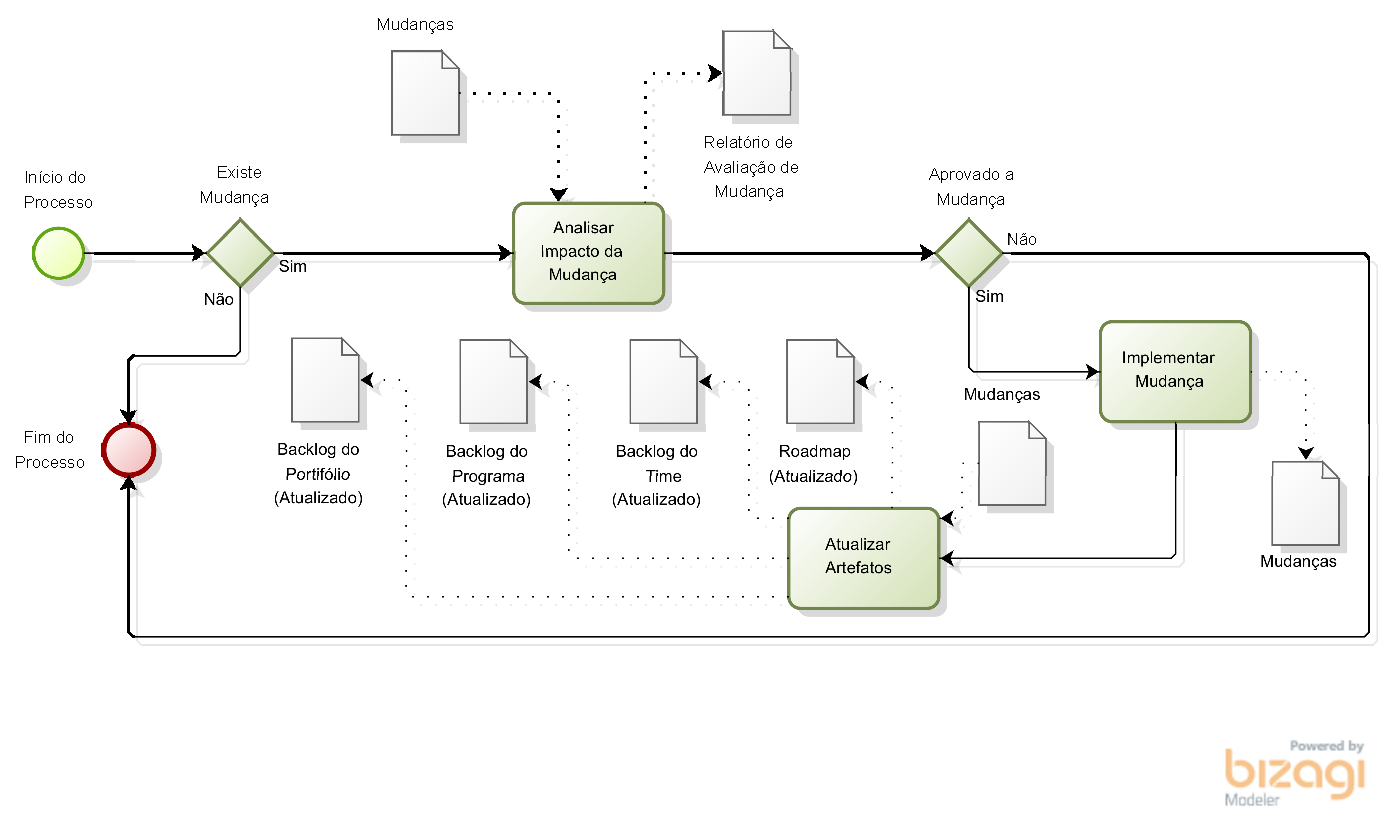
\includegraphics[keepaspectratio=true,scale=0.5]{figuras/gerencia.eps}
    \caption{Gerência de Mudança}
    \label{fig:processo}
\end{figure}